%%%%%%%%%%%%%%%%% DO NOT CHANGE HERE %%%%%%%%%%%%%%%%%%%% {
\documentclass[12pt,letterpaper]{article} \usepackage{fullpage}
\usepackage[top=2cm, bottom=4.5cm, left=2.5cm, right=2.5cm]{geometry}
\usepackage{amsmath,amsthm,amsfonts,amssymb,amscd}
\usepackage{lastpage}
\usepackage{enumerate}
\usepackage{fancyhdr}
\usepackage{mathrsfs}
\usepackage{xcolor}
\usepackage{graphicx}
\usepackage{listings}
\usepackage{hyperref}

\hypersetup{%
    colorlinks=true,
    linkcolor=blue,
    linkbordercolor={0 0 1}
}

\setlength{\parindent}{0.0in}
\setlength{\parskip}{0.05in}
%%%%%%%%%%%%%%%%%%%%%%%%%%%%%%%%%%%%%%%%%%%%%%%%%%%%%%%%%% }

%%%%%%%%%%%%%%%%%%%%%%%% CHANGE HERE %%%%%%%%%%%%%%%%%%%% {
\newcommand\course{Ilya Sherstyuk}
\newcommand\semester{Spring 2021}
\newcommand\hwnumber{2}                 % <-- ASSIGNMENT #
%%%%%%%%%%%%%%%%%%%%%%%%%%%%%%%%%%%%%%%%%%%%%%%%%%%%%%%%%% }

%%%%%%%%%%%%%%%%% DO NOT CHANGE HERE %%%%%%%%%%%%%%%%%%%% {
\pagestyle{fancyplain}
\headheight 35pt
\lhead{\NetIDa}
\lhead{\NetIDa\\\NetIDb}
\chead{\textbf{\Large CS 148 Set \hwnumber}}
\rhead{\course \\ \semester}
\lfoot{}
\cfoot{}
\rfoot{\small\thepage}
\headsep 1.5em
%%%%%%%%%%%%%%%%%%%%%%%%%%%%%%%%%%%%%%%%%%%%%%%%%%%%%%%%%% }

\begin{document}

% \begin{flushright}Collaborator: Elise Liu\end{flushright}

\textbf{1. Algorithms description}

My algorithm consisted of scanning template arrays over the input image and
making a heatmap array recording the dot products at each location. Then, the
heatmap was converted into a list of detections.\\\\
To make the templates, I chose ten images of traffic lights of various colors and
sizes from the training data. I then converted them into numpy arrays and
normalized them with respect to their source image. Each color channel was
normalized separately. These numpy arrays are saved as templates. \\\\
The detection algorithm is as follows:

\begin{enumerate}
    \item Normalize each color channel of the input image to have 0 mean and
    unit standard deviation.
    \item For each kernel (template), convolve it with the normalized image to create
    a heatmap for that kernel.
    The convolution uses zero-padding.
    The stride was set to roughly 1/5th the kernel
    width. The resulting heatmap is scaled to have the same size as the input image.
    The values in the heatmap are divided by the kernel area in an attempt to
    account for kernel size (so larger kernels won't produce stronger heatmaps).
    \item The resulting heatmap of the image is the pixelwise max of each kernel
    heatmap.
    \item Set $T = 2.5$ to be the threshold. Note which pixels in the heatmap
    have value greater than $T$. Divide these pixels into groups based on adjacency.
    For each group, create a bounding box with each dimension extending
    to the furthest pixel in that group. Call $v$ the maximum pixel value in the group,
    and set the confidence of that detection to \[C = \frac{1}{1+2^{-v}}\]
    This is to ensure that the confidence falls between 0 and 1.
    \item Return the bounding boxes and their corresponding confidence levels.
\end{enumerate}


\textbf{2. Templates}

\begin{figure}[htp]
    \centering
    
\includegraphics[width=1cm]{../templates/red-light/RL-001.jpg}
    
\includegraphics[width=1cm]{../templates/red-light/RL-010.jpg}
    
\includegraphics[width=1cm]{../templates/red-light/RL-016.jpg}
    
\includegraphics[width=1cm]{../templates/red-light/RL-028.jpg}
    
\includegraphics[width=1cm]{../templates/red-light/RL-042.jpg}
    
\includegraphics[width=1cm]{../templates/red-light/RL-050.jpg}
    
\includegraphics[width=1cm]{../templates/red-light/RL-107.jpg}
    
\includegraphics[width=1cm]{../templates/red-light/RL-116.jpg}
    
\includegraphics[width=1cm]{../templates/red-light/RL-134.jpg}
    
\includegraphics[width=1cm]{../templates/red-light/RL-213.jpg}
\end{figure}

Above are the template images. A few things to note:
\begin{itemize}
    \item First, the templates are not all the same size like they are shown
    in this document. They were selected to cover a large range of sizes, to
    match as many different sizes of traffic lights as possible, as
    they are not rescaled in the algorithm.
    \item Second, these are not actually the exact templates. The templates
    are arrays which were created from the above images and then normalized with
    respect to the source image. So the templates also in a sense contain information
    about what a traffic light should look like compared to the rest of the image.
\end{itemize}

I already described how I localized the box locations in the algorithm above but I'll
briefly go over it again here. All of the templates were convolved with the source
image to create heatmaps, and the heatmaps were combined into one by taking the maximum
of each pixel over the heatmaps. Pixels which crossed a threshold value were selected
as detections, and adjacent detections were combined into one.\\\\
Here is a cool visualization of the heatmaps for a couple of the test images:
\begin{figure}[htp]
    \centering
    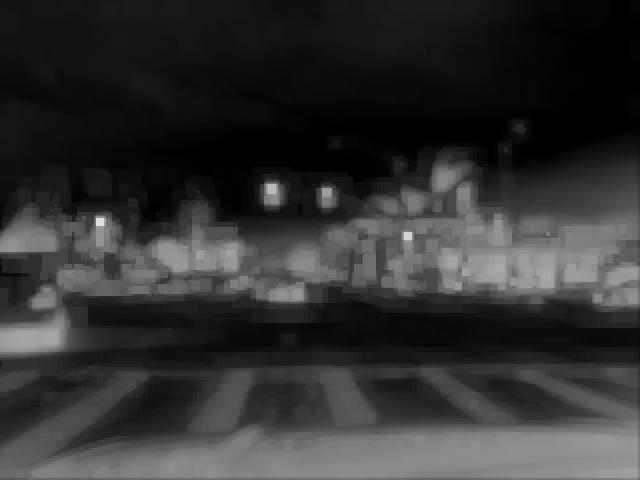
\includegraphics[width=8cm]{img/heatmap-196.jpg}
    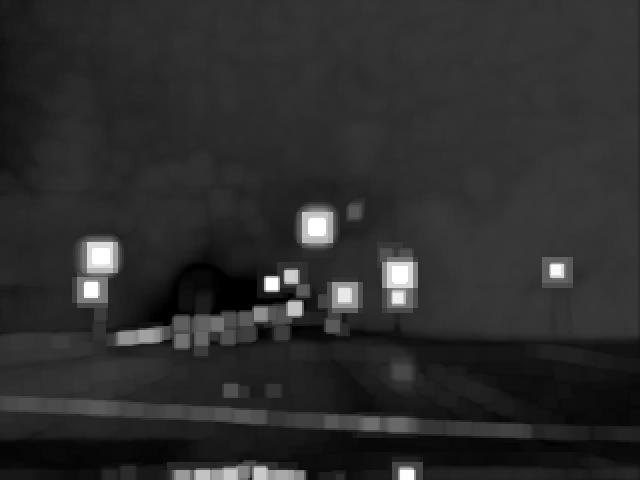
\includegraphics[width=8cm]{img/heatmap-334.jpg}
\end{figure}\\
You can tell that the heatmaps are brightest around traffic lights and similar
objects.
\\\\
\textbf{3. Good Examples}
\begin{figure}[htp]
    \centering
    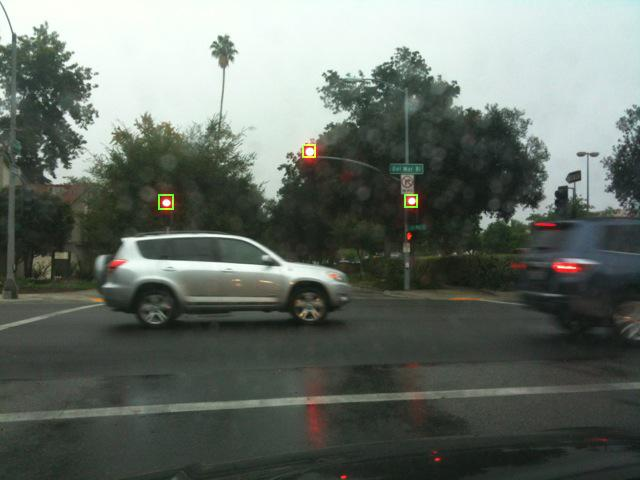
\includegraphics[width=8cm]{img/RL-049.jpg}
    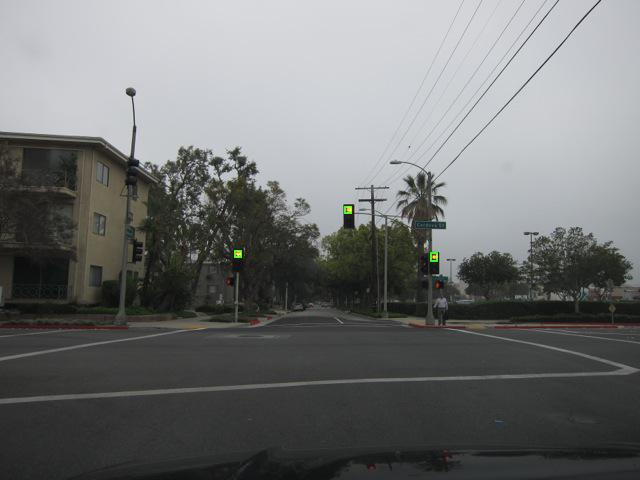
\includegraphics[width=8cm]{img/RL-271.jpg}
\end{figure}
Here are two examples from the test set where my algorithm succeeded.
The bounding boxes are drawn in green.\\
I think these images were easy for my algorithm because the traffic lights were
fairly close to the camera and similar to the template images. The fact that they are large makes
it easier for the templates to overlap with them, and of course being similar to the
templates is helpful too.
\\\\
\textbf{4. Bad Examples}

\begin{figure}[htp]
    \centering
    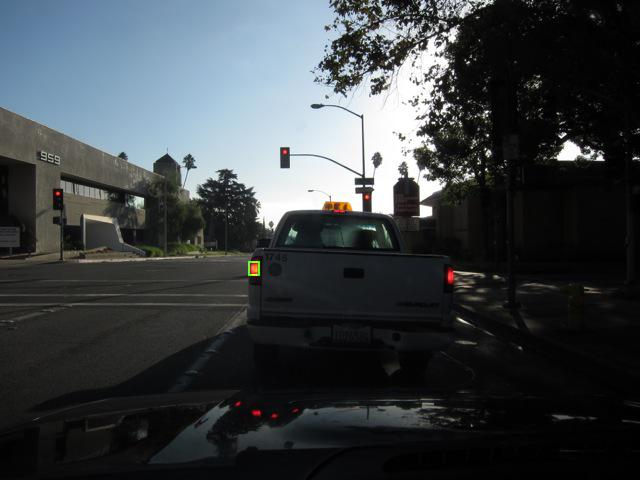
\includegraphics[width=8cm]{img/RL-021.jpg}
    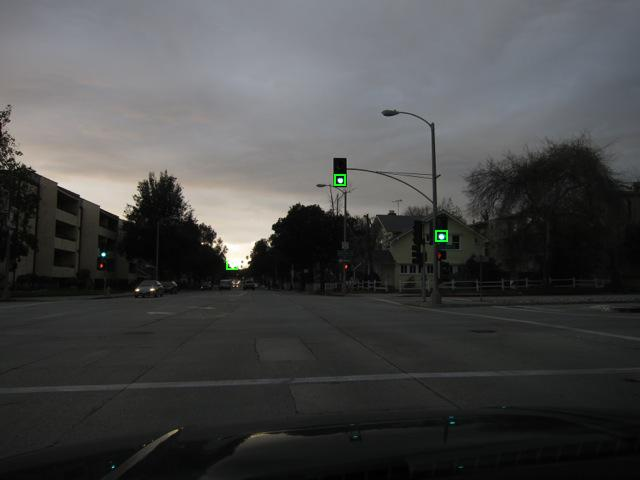
\includegraphics[width=8cm]{img/RL-204.jpg}
\end{figure}

Here are two examples from the test data where my algorithm failed.\\

On the left, we see that the algorithm failed missed the traffic lights and instead
opted for the truck's brake light. I think the reason why this image failed was because
it was very dark. I selected templates of traffic lights when it was dark, but in those
templates the traffic light had always been very bright, but in this image both
the image and the traffic lights are dim. However, the truck's brake light is quite bright,
so the algorithm must have liked that.\\

On the right, we see that it incorrectly detected the green traffic lights. I think the
failure here was caused by a lack of contrast in the image. Because there is very little
red color in this image, when the image is normalized by channel, it doesn't have an actual
red part of the image to normalize against. Thus, it might pick up bright spots of colors
which are not actually red.

\newpage
\textbf{5. P-R Plot}\\
\begin{figure}[htp]
    \centering
    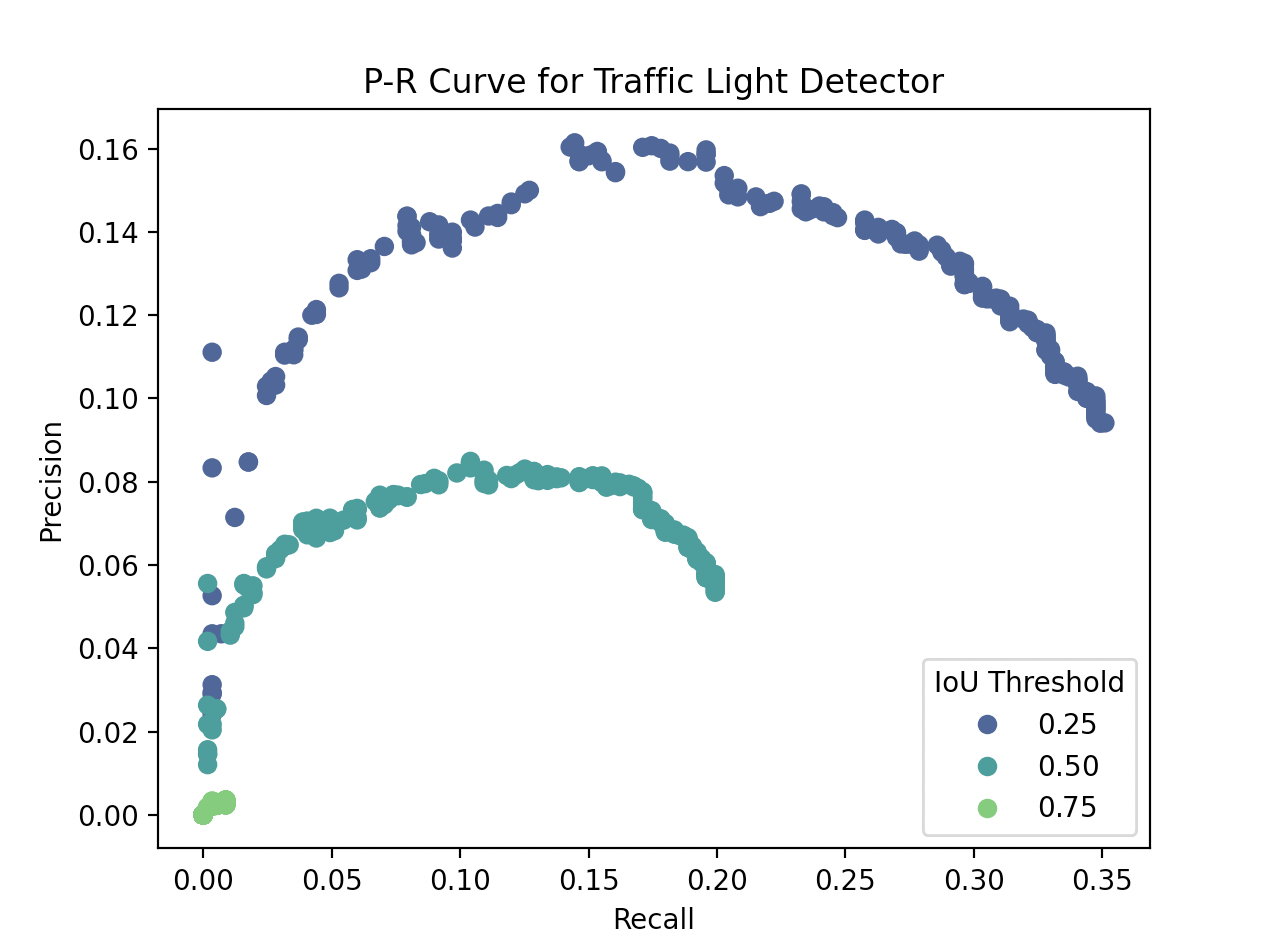
\includegraphics[width=8cm]{img/pr-train.png}
    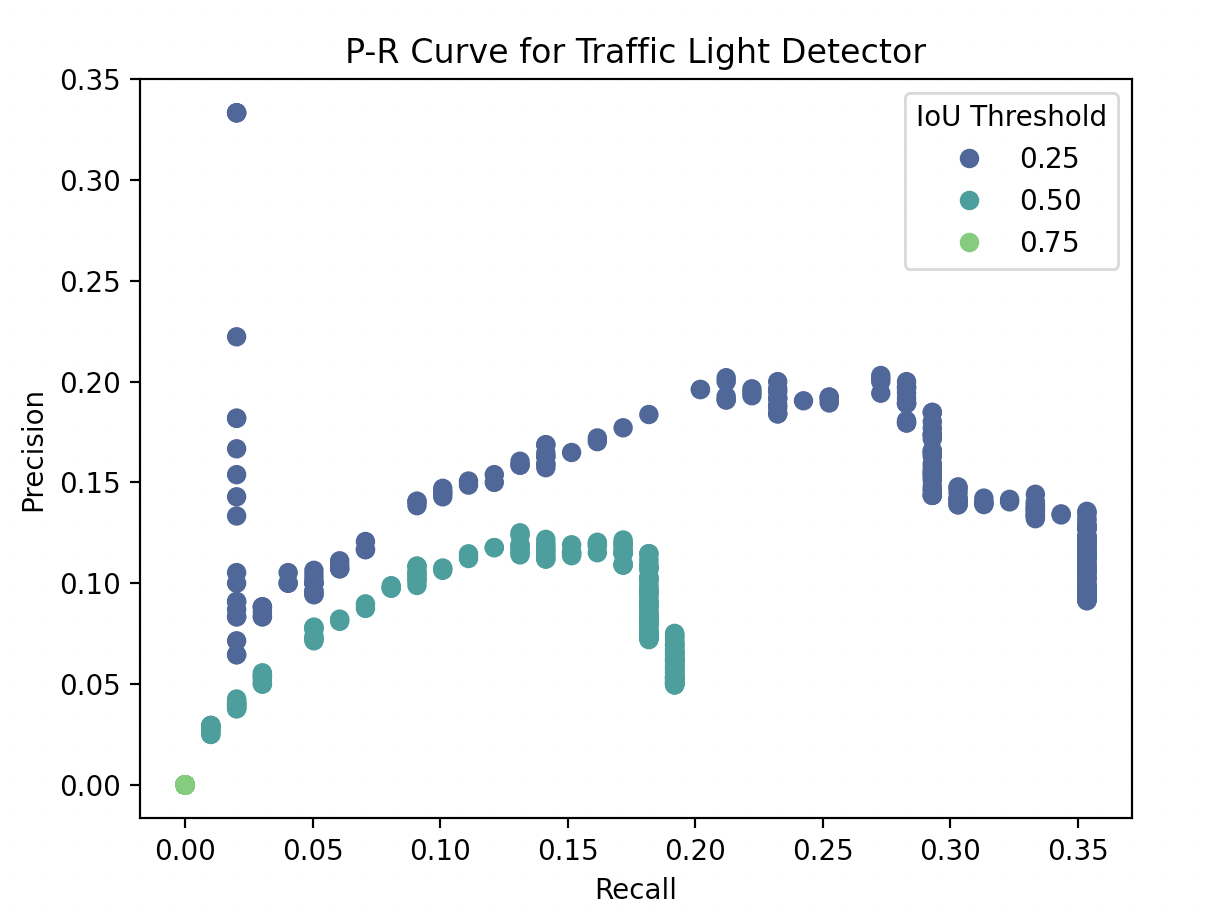
\includegraphics[width=8cm]{img/pr-test.png}
\end{figure}
Here are the Precision-Recall Curves for the training set (left) and the test set (right).
As you can see, increasing the IoU threshold decreases both the precision and the accuracy,
which makes sense because we are limiting the number of detections. The train curve has a
lot more points, but besides that the curves are pretty similar. We can see though that
for a given IoU threshold, the test set seems to perform better (the frontier of the curve
has a higher precision for the given recall). This shows us that we didn't overfit our
algorithm to the training set.
\\\\
For my ``weakened'' algorithm, I cut the number of templates down to 4. Besides that,
the algorithm is the same. Here are the Precision-Recall curves for the weakened algorithm:\\
\begin{figure}[htp]
    \centering
    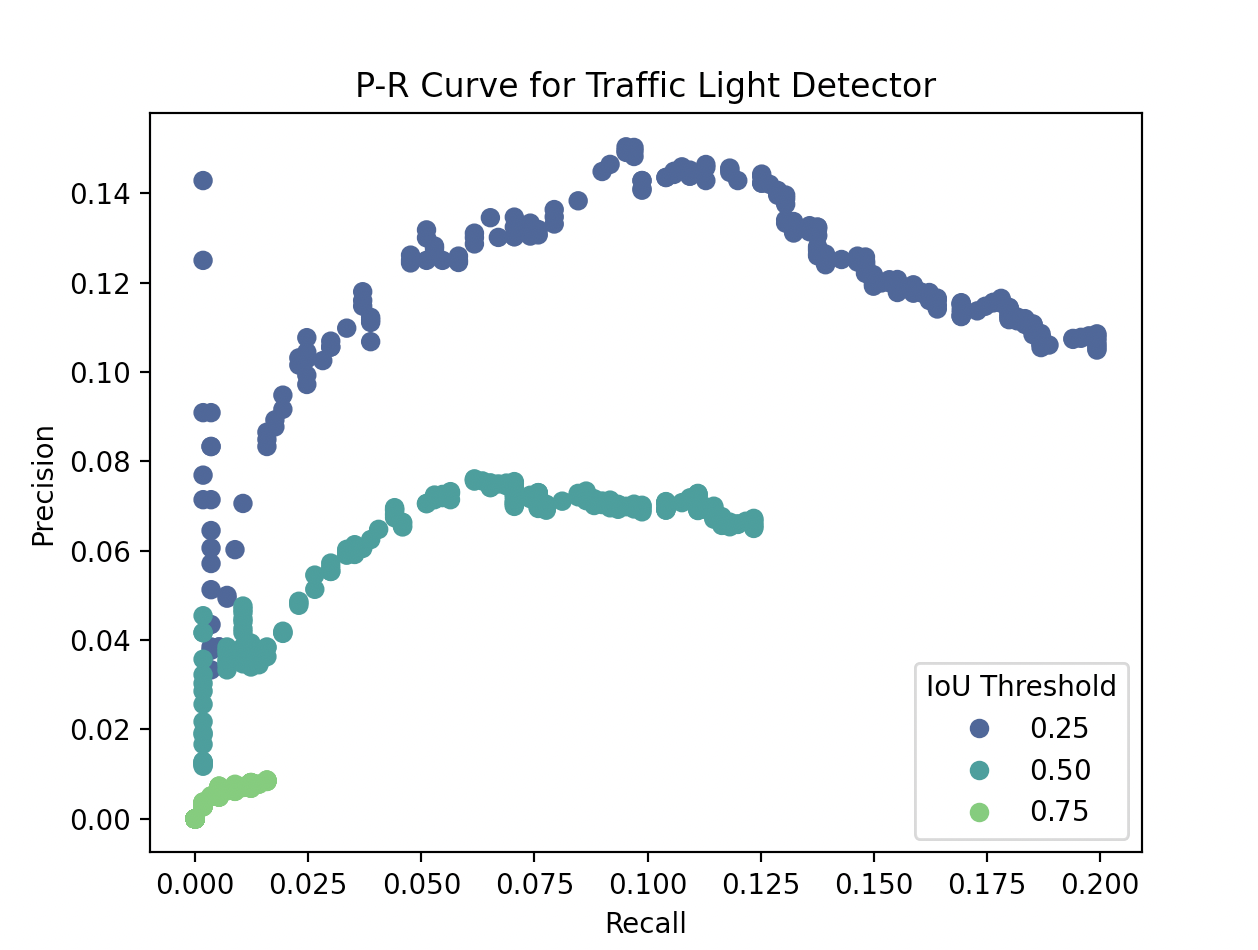
\includegraphics[width=8cm]{img/pr-train-weak.png}
    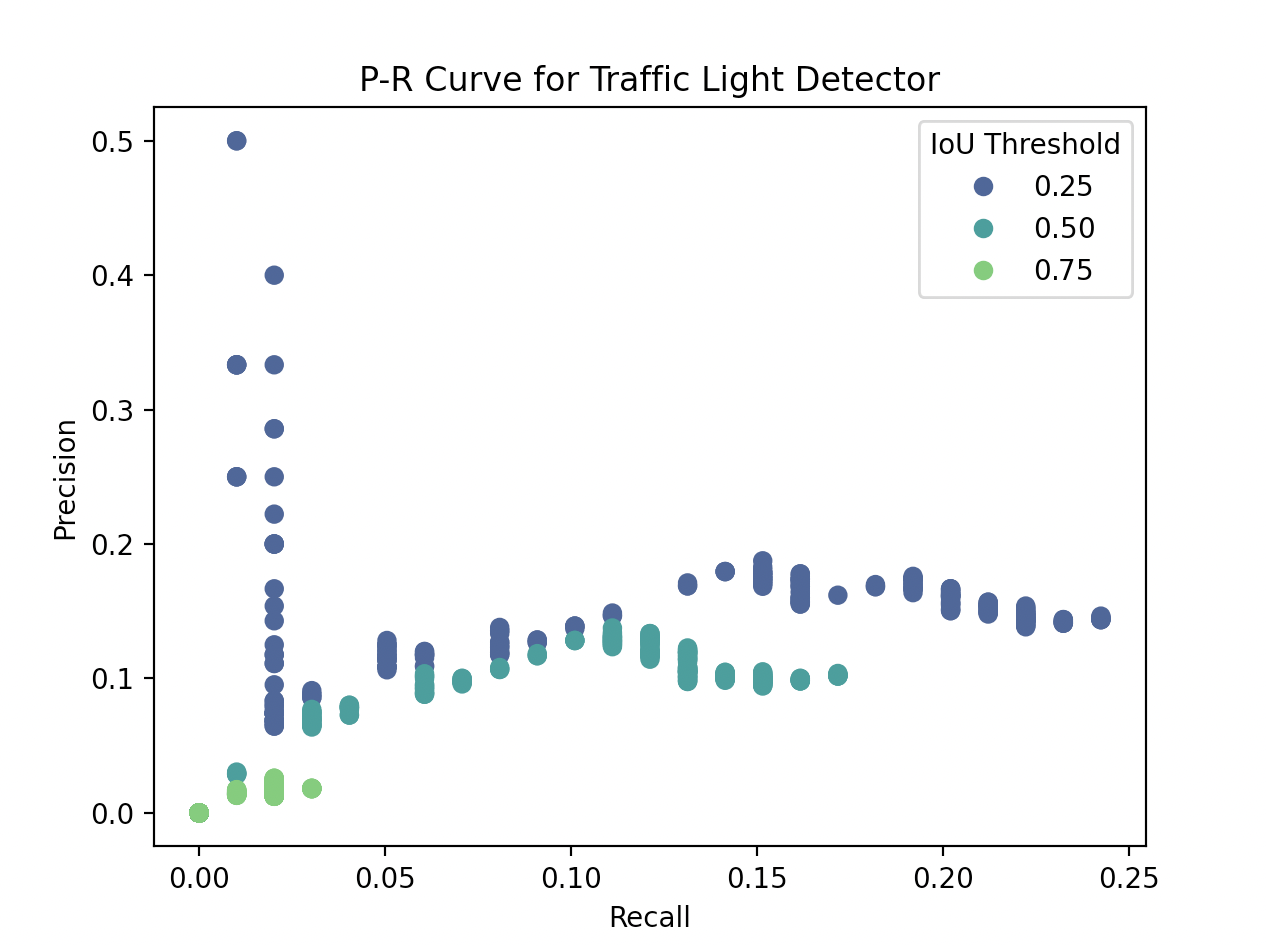
\includegraphics[width=8cm]{img/pr-test-weak.png}
\end{figure}
As you can see, the recall is much lower in this ``weakened'' algorithm for a given
precision level compared to the full algorithm. This makes sense, since I am giving the
algorithm fewer examples of what traffic lights look like in this weakened version.
\\\\
It is useful to compare the algorithm to a weaker version because that allows you to test
whether how much each of the complications actually make a difference in the end. For example,
you might discover that a certain feature of the algorithm is critically important, while
another one is actually detrimental to the performace. In this case, I can see that my
five extra templates were actually helpful with the recall of the algorithm.\\


\textbf{Deliverable \#3}

Repo Link: \url{https://github.com/ilyasher/caltech-ee148-spring2020-hw02}

The code for the algorithm is in run\_predictions.py and the script
to generate the PR curves is called eval\_detector.py

\end{document}
